\chapter {Preliminaries}
\label{chp:pre}

In my dissertation, I will study triangle listing problem for web-scale graphs and anonymization techniques in the context of uncertain graphs. For the later topics, we focus on resisting the degree-based node re-identification. Here, we give the definitions of uncertain graph model and attack model, privacy criteria related with uncertain graph anonymization problem. We also give the formal formulation of proposed problems. 

\section{Distributed Triangle Listing}
\subsection{Triangle Listing Problem}
Suppose we have a simple undirected graph $G(V,E)$, where $V$ is the set of vertices (nodes), and $E$ is the set of edges. Let $n=|V|$ and $m=|E|$. Let $N_v = \{u | (u,v) \in E \}$ denote the set of \emph{adjacent nodes} of node $v$, and $d_v=|N_v|$ denote the degree of node $v$. We assume that  $G$ is stored in the most popular format for graph data, {\ie}, the adjacency list representation. Given any three distinct vertices $u, v, w \in V$, they form a triangle $\triangle_{uvw}$, iif $(u,v), (u,w), (v,w) \in E$. We define the set of all triangles that involve node $v$ as $\triangle(v)=\{ \triangle_{uvw} | \  (v,u), (v,w), (u,w) \in E \}$. Similarly, we define $\triangle(G)= \bigcup_{v \in V} {\triangle (v)}$ as the set of all triangles in $G$.

\begin{problem}
    \textbf{Triangle Listing Problem}: Given a  large-scale distributed graph $G(V,E)$, our goal is to report all triangles in $G$, {\ie}, $\triangle(G)$, in a highly distributed way. 
    \label{prob:TLMap}
\end{problem}

\subsection{Sequential Triangle Listing}
\label{sec:InMemoryAlgorithms}
\begin{algorithm}[t]
    \begin{algorithmic}[1]
        \item[] {\textbf{Preprocessing step}} 
        \FORALL{$(u,v) \in E$}
            \STATE {if $u \succ v$, store $u$ in $N_v^H$}
            \STATE {else store $v$ in $N_u^H$}
         \ENDFOR
        \item[] {\textbf{Triangle Listing}}
        \STATE{$\triangle(G) \leftarrow \emptyset $}
        \FORALL{$v \in V$}
            \FORALL{$u \in N_v^H$}
                \FORALL{ $w \in N_v^H \bigcap N_u^H$}
                    \STATE{$\triangle(G) \leftarrow \triangle(G) \bigcup \lbrace \triangle_{vuw} \rbrace$}
                 \ENDFOR
            \ENDFOR
        \ENDFOR
    \caption{NodeIterator++}
    \label{alg:Node}
    \end{algorithmic}
\end{algorithm}
Sequentail triangle listing algorithms have been extensively stuidied. Here, we present a sequential triangle listing algorithm which is widely used as the basis of parallel approaches \cite{Suri_Vassilvitskii_2011,Patric,parkmapreduce2014}. In this work, we also use it as the basis of our distributed approach. 

A naive algorithm for listing triangles is as follows. For each node $v \in V$, find the set of edges among its neighbors, i.e., pairs of neighbors that complete a triangle with node $v$. Given  this simple method, each triangle $(u,v,w)$ is listed six times---all six permutations of $u$, $v$ and $w$. Several other algorithms have been proposed to improve on and eliminate the redundancy of this basic method, e.g.,~\cite{Schank_2007,Becchetti_Boldi_Castillo_Gionis_2008}.

One of the algorithms, known as \emph{NodeIterator++}~\cite{Schank_2007}, uses a total ordering over the nodes to avoid duplicate listing of the same triangle. By following a specific ordering, it guarantees  that each triangle is counted only once among the six permutations. Moreover, the NodeIterator++ algorithm  adopts an interesting node ordering based on the nodes'  degrees, with ties broken by node IDs, as defined blow: 
\begin{equation*}
    u \succ v \Longleftrightarrow d_u > d_v ~or~(d_u=d_v ~and ~u>v)
    \label{eq:totalOrder}
\end{equation*}
% \vspace{-1em}
This degree-based ordering improves the running time by reducing the diversity of the effective degree $\hat{d_v}$. The running time of NodeIterator++ algorithm is $O(m^{3/2})$. A comprehensive analysis  can be found in~\cite{Schank_2007}.

The standard \emph{NodeIterator++} algorithm performs the degree-based ordering comparison during the final phase, i.e., the triangle listing phase. 
The work in~\cite{Patric} and~\cite{Suri_Vassilvitskii_2011} further improves on that by performing the comparison $u \succ v$ for each edge $(u,v) \in E$ 
in the preprocessing step (Lines 1-3, Algorithm~\ref{alg:Node}). For each node $v$ and edge $(u,v)$, node $u$ is stored in the effective list of $v$ ($N_v^H$) 
if and only if $u \succ v$, and hence $N_{v}^H=\lbrace u: u\succ v ~and~ (u,v) \in E \rbrace$. 
The preprocessing step cuts the storage and memory requirement by half since each edge is stored only once. After the preprocessing step, the effective degree of nodes in $G$ is $O(\sqrt[]{m})$~\cite{Schank_2007}. Its correctness proof can be found in \cite{Patric}.
The modified NodeIterator++ algorithm is presented in Algorithm~\ref{alg:Node}. 

\subsection{MapReduce Overview}
MapReduce is a popular distributed programming framework for processing large datasets~\cite{MapReduceGoogle}. 
MapReduce, and its open-source implementation Hadoop~\cite{whitehadoop_2010}, have been used for many important 
graph mining tasks~\cite{Suri_Vassilvitskii_2011,parkmapreduce2014}. 
In this paper, our algorithms are designed and analyzed in the MapReduce framework. 

\textbf{Computation Model.} An analytical  job in MapReduce executes in two rigid phases, called the {\em map} and {\em reduce} phases. Each phase consumes/produces records in the form of {\em key-value} pairs---We will use the keywords {\em pair}, {\em record}, or {\em message} interchangeably to refer to these key-value pairs. 
A pair is denoted as $\langle k;val \rangle $, where $k$ is the key and $val$ is the value. 
The {\em map} phase takes one key-value pair as input at a time, and produces zero or more output pairs. 
The {\em reduce} phase receives multiple key-listOfValues pairs and produces zero or more output pairs. 
Between the two phases, there is an implicit phase, called {\em shuffling/sorting}, in which the mappers' output pairs are 
 shuffled and sorted to group the pairs of the same key together as input for reducers. 

Our proposed solution will leverage and extend some of the basic functionality of MapReduce, which are:
\begin{itemize}
\item {{\bf Key Partitioning:} 
        Mappers employ a \emph{key partitioning function} over their outputs to partition and route the records across the reducers. 
        By default, it is a hash-based function, but can be replaced by any other user-defined logic. 
%       \SysName will make use of the partitioning function to proactively learns where and when each node/key will be processed, and hence minimize the communication overhead.
}
\item {{\bf Multi-Key Reducers:} 
    Typically, the number of distinct keys in an application is much larger than the number of reducers in the system. 
    This implies that a single reducer will sequentially process multiple keys---along with their associated groups of values---in the same reduce instance. 
      Moreover, the processing order is defined by \emph{key sorting function} used in shuffling/sorting phase. 
    By default, a single reduce instance processes each of its input groups in total isolation from the other groups with no sharing or communication. 
 }  
\end{itemize}

\subsection{Triangle Listing in MapReduce}
\label{sec:MR_baseline}
\begin{algorithm}[t]
    \begin{algorithmic}[1]
                \item[] {\textbf{Map}: Input: $\langle v;N_v^H \rangle$}
                \STATE emit $\langle v;(v,N_v^H) \rangle$
                \FORALL {$u \in  N_v^H$}
                    \STATE emit $\langle u;(v,N_v^H) \rangle$
                \ENDFOR
                \item[]
                \item[]\textbf{Reduce}:Input:$[ \langle u;(v,N_v^H) \rangle ]$ 
                \STATE initiate $N_u^H$  
                \FORALL {$\langle u;(v,N_v^H) \rangle $}
                    \FORALL {$w \in N_u^H \cap N_v^H $}
                        \STATE emit $\triangle_{vuw}$
                    \ENDFOR
                \ENDFOR
                 \caption{MR-Baseline}
                \label{alg:MR-Baseline}
      \end{algorithmic}
\end{algorithm}
Both \cite{Suri_Vassilvitskii_2011} and \cite{Patric} use the NodeIterator++ algorithm as the basis of their distributed algorithms.\cite{Suri_Vassilvitskii_2011} identifies the triangles by checking the existence of pivot edges, while \cite{Patric} uses set intersection of effective adjacency list (Line 7, Algorithm \ref{alg:Node}). In this section, we present the MapReduce version of the NodeIterator++ algorithm similar to the one presented  in \cite{Patric},  
referred to as {\em MR-Baseline} (Algorithm~\ref{alg:MR-Baseline}). 

The general approach is the same as in the NodeIterator++ algorithm. In the map phase, each node $v$ needs to emit two types of messages. The first type is used for the initiation its own effective adjacency list in the reduce side, 
referred to as {\em a core message} (Line 1, Algorithm \ref{alg:MR-Baseline}). 
The second type is used for identifying triangles, referred to as {\em pivot messages} (Lines 2-3, Algorithm \ref{alg:MR-Baseline}). 
All pivot messages from $v$ to its effective adjacent nodes are identical. In the reduce phase, each node $u$ will receive a core message from itself, and a pivot message from adjacent nodes with the lower degree. Then, each node identifies the triangles by performing a set intersection operation (Lines 5-6, Algorithm \ref{alg:MR-Baseline}). 

We omit the code of the pre-processing procedure since its implementation is straightforward in MapReduce. In addition, we will exclude the pre-processing cost for any further consideration since it is typically dominated by the actual running time of the triangle listing algorithm, plus it is the same overhead for all algorithms. 

\section{Privacy Protection on Uncertain Graphs}
\subsection{Uncertain Graph}
Let  $\mathcal{G}=(V,E,\mathit{p})$ be an uncertain graph, where $V$ is the set of nodes, $E$ is the set of edges, and function $\mathit{p}: E \rightarrow [0,1]$ assigns a  probability of existence to each each edge, denoted as $\mathit{p}(e)$. We consider the edge probabilities are independent, and we assume \emph{possible world} semantics, consistent with existing literature~\cite{Potamias_K_2010,Adar_Managing_2007,Kempe_Maximizing_2003}. Specifically, the \emph{possible world} semantics interprets $\mathcal{G}$ as a set of possible deterministic graphs $W(\mathcal{G})$, each deterministic graph $G \in W(\mathcal{G})$ including all vertices of $\mathcal{G}$ and a subset of edges $E_{G} \subset E$.  The probability of observing any possible world $G=(V,E_{G}) \in W(\mathcal{G})$ is 
\begin{equation*}
    Pr[G]=\prod_{e \in E_{G}} {\mathit{p}(e)} \prod_{e \in E     \setminus E_{G}} (1-\mathit{p}(e))
\end{equation*}
We can think of the uncertain graph $\mathcal{G}$ as a world generator process, and each graph $G\in W(\mathcal{G})$ as a possible world. 

\subsection{Attack Model}
\begin{figure*}[t!]
    \centering
    \begin{subfigure}[t]{0.4\textwidth}
        \centering
        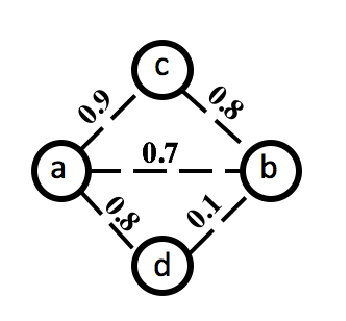
\includegraphics[scale=0.6]{figures/DegreeAUG/trueGraph.eps}
        \caption{\small{An \emph{original} graph.}}
         \label{fig:trueGraph}
    \end{subfigure}
    \begin{subfigure}[t]{0.4\textwidth}
        \centering
        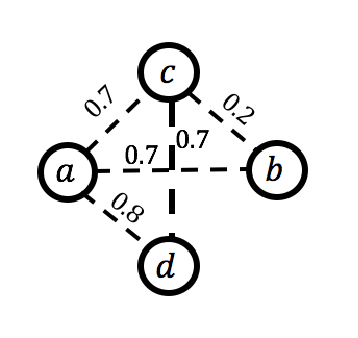
\includegraphics[scale=0.6]{figures/DegreeAUG/anGraph.eps}
        \caption{\small{An \emph{anonymization}.}}
        \label{fig:anGraph}
    \end{subfigure}
    \caption{Uncertain graph anonymization.}
    \label{fig:augExample}
\end{figure*}
Uncertain graph anonymization problem is related to the conventional graph anonymization problem, which has been extensively studied. As Hay {\etal} pointed out, the structural information such as node degree, 1-neighbood can be utilized to breach user privacy. For example, \cite{Boldi_Injecting_2012,Liu_Towards_2008,Thompson_The_2009} consider the case that a vertex can be re-identified by its degree, while \cite{Cormode_Anonymizing_2008,Wu_k_2010} consider the case that a vertex can be re-identified by degrees of it and its neighbood. Different anonymization techniques are designed to resist different kinds of privacy attack.

The first step to anonymization is to know what external information of a graph may be acquired by an adversary. In our work, we assume that the information of victim node degree is easy to be collected by the adversary, consistent to the literture~\cite{Liu_Towards_2008,Thompson_The_2009,Boldi_Injecting_2012,Wu_k_2010,Cormode_Anonymizing_2008}.  In fact, degree-based de-anonymization is one of the most serious privacy attacks in the context of deterministic graphs. The knowledge  could also be understood as some \emph{assertion} of the individual, which could be evaluated to \emph{true} or \emph{false} based on the topology structure of the network. 

In the context of deterministic graphs, such knowledge can be expressed as one assertion with certainty such as {\emph Ana has 3 neighbors. In the context of uncertain graphs, such knowledge can be a little different. Given an uncertain graph $\mathcal{G}$, let the degree of a fixed node $v$ to be $d_{v}$, clearly the observation of $d_{v}$ differs on the possible worlds $G \in W(\mathcal{G})$. We define the $d_{v}$ as a random variable with a known distribution. We base our degree-related adversary knowledges on standard stastical measures of the distribution. 

It is difficult to model the specific degree-related knowledge used by the adversaries by advance. In our work, we first consider the adversary can and only acquire the expected node degree of victim nodes. For example, the adversary knows that the expected value of the number of Ana's neighbors should $3$  as shown in Figure \ref{fig:trueGraph}.  Later, we consider the adversary can acquire more comprehensive knowledge of node degree of victim nodes such as the distribution function. For example, the adversary may know the distribution of the number of Ana's neighbors as ${(3:0.504),(2:0.398),(1:0.092),(0:0.006)}$. 

The second step to anonymization is to know how the adversary links the external knowledge such as node degree to a node in the perturbed graph. In the deterministic graph, the process of node de-anonymization with the external node degree information is quite straightforward. Let $\mathcal{G}$ be a graph and $\acute{\mathcal{G}}$ be the anonymized version of the given graph. The adversary can get a number of \texttt{match} vertices in $\acute{\mathcal{G}}$, {\ie}, the nodes $U_{c}$ with the \texttt{match} degree. When $\acute{\mathcal{G}}$ is a deterministic one, for a given node in $\acute{\mathcal{G}}$, the assertion is evaluated either \emph{true} or \emph{false} with certainty. When the anonymized output $\acute{\mathcal{G}}$ is probabilistic one, the matching attack is performed over all the possible worlds. Following the path, the matching event would be observed with an probability value which defined in a continous range $(0,1)$. For example, the probability that the node $a$ was observed with degree $3$ is $0.504$ in Figure \ref{}. We consider the matching attack is performed between a random variable, namely, find the equal random variable. Namely, for a given node $u$ in $\acute{\mathcal{G}}$, it is defined as the probability that the random variable $d_{u}$ is equal to the adversary knowledge $d_{v}$, denotes as $P(d_{u}=d_{v})$. It can be computed as 
\begin{equation*}
    P(d_{u}=d_{v})= \sum_{i \in Z } P(d_{u}=i) P(d_{v}=i) 
\end{equation*}

%%%
\subsection{Privacy Criteria}
As ever discussed, we want to publish the anonymized version of uncertain graphs where node identity is obfuscated enough. We adopt $\keobf$ model, proposed in \cite{Bonchi_Identity_2014}, to quantify the anonymity level achieved by an anonymized graph (uncertain graph).
Its formal definition is as follow: 
\begin{definition}
    \textbf{\boldmath{$(k,\epsilon)$}-obf \cite{Bonchi_Identity_2014}}
    Let $P$ be a vertex property, $k \geq 1$ be a desired level of anonymity, and $\epsilon >0 $ be a tolerance parameter. The uncertain graph $\tilde{\mathcal{G}}$ is said to $k$-obfuscate a given vertex $v \in V_{\mathcal{G}}$ with respect to $P$ if the entropy of the distribution $Y_{P(v)}$ over the vertices of $\mathcal{G}$ is greater than or equals to $\log_{2}{k}$:
    \vj
    \begin{equation*}
        H(Y_{P(v)}) \geq \log_{2}{k}.
    \label{obfCon}
    \svj
    \end{equation*}
The uncertain graph $\mathcal{G}$ is $(k,\epsilon)$-obf with respect to property $P$ if it $k$-obfuscates at least $(1-\epsilon)|V|$ vertices in $V_{\mathcal{G}}$. $P$ can be any node properties.  
\end{definition}

\begin{figure}[t]
        \centering    
        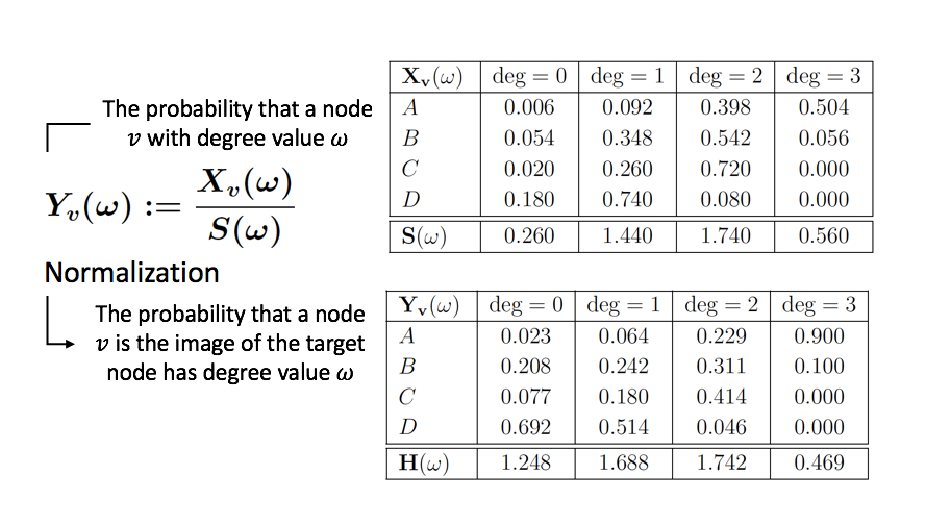
\includegraphics[scale=0.8]{figures/DegreeAUG/entropyEx.eps}
        \caption{The degree uncertainty for each node (top) and normalized values for each degree (bottom)}
    \label{fig:entropyExample}
\end{figure}

\emph{Figure \ref{fig:entropyExample}  gives an example of how to compute degree entropy for the uncertain graph in Figure \ref{fig:trueGraph}. Each row in the top side is the degree distribution for the corresponding node. For example, node $a$ has degree $0$ with probability $(1-0.9)(1-0.8)(1-0.7)=0.006$. The last row in the top side is the sum of probability over all the nodes. For example, $S(0)=0.006+0.054+0.020+0.180=0.26$.
The bottom one normalizes values in each column to get distribution $Y_{P(v)}$. For example, $Y_{0}(a)$= $\frac{X_{0}(a)}{S(0)}=0.023$. The entropy $H(Y_d(v))$ for each degree value $\omega$ is shown in the last bottom row. Given $k=3, \log_{2}{3}=1.58$, node $b,c$ with expected degree $2$ and $d$ with true degree $1$ satisfies $k$-obf while $a$ with expected degree $3$ fails, thus $\epsilon=0.25$.}

\subsection{Reliability-based Utility Criteria}
Inspired by the importance of reliability, we suggest to quantify the utility loss, anonymization cost, as the reliability difference between the anonymized result $\tilde{\mathcal{G}}$ and the original one $\mathcal{G}$, reliability discrepancy. We proceed to explain its formal definition. 

In the context of uncertain graphs, \emph{reliability} generalizes the concept of connectivity by  capturing the probability that two given (sets of) nodes are reachable over all possible worlds. We focus on two-terminal reliability. 
\begin{definition}
    \textbf{Two-Terminal Reliability \cite{Colbourn_Colbourn_1987}}  Given an uncertain graph $\mathcal{G}$, and two distinct nodes $u$ and $v$ in $V$, the reliability for two nodes $(u,v)$ is defined as follows:
        \vj
        \begin{equation*}
                R_{u,v}(\mathcal{G})= \sum_{G \subseteq W(\mathcal{G})}  \mathcal{I}_{G}(u,v) Pr[G] 
        \svj
        \end{equation*}
     
    where $\mathcal{I}_{G}(u,v)$ is 1 when $u$ and $v$ are contained in a connected component in $G$, and 0 otherwise.     
    \label{d:reliability}
\end{definition}

\begin{definition}
    \textbf{Two-Terminal Reliability Discrepancy}
    The reliability discrepancy of two distinct nodes $(u,v)$ is defined as the absolute difference of  corresponding reliability values in the original graph $\mathcal{G}$ and the anonymized result $\tilde{\mathcal{G}}$. Its formal definition is as follows:  
    \begin{equation*}
    RD_{u,v}(\tilde{\mathcal{G}})= |R_{u,v}(\mathcal{G})-R_{u,v}(\tilde{\mathcal{G}})|
    \end{equation*}
\end{definition}
Thus, we come up the definition of reliability discrepancy of the overall anonymized result against the true graph.   
\begin{definition}
    \textbf{Reliability Discrepancy}
    Compared to the input uncertain graph $\mathcal{G}=(V,E,\mathit{p})$, the reliability discrepancy of one anonymized instance $\tilde{\mathcal{G}}=(V,E, \tilde{\mathit{p}})$ is the sum of $RD$ over all vertex pair $(u,v)$. The formal definition is as follows: 
    \begin{equation*}
        \Delta(\tilde{\mathcal{G}})=\sum_{(u,v)} RD_{u,v}(\tilde{\mathcal{G}})
    \end{equation*}
\end{definition}

\begin{example}
 Given an input uncertain graph $\mathcal{G}$ in Figure \ref{fig:trueGraph} and its anonymization $\tilde{\mathcal{G}}$ in Figure \ref{fig:anGraph} and suppose one wants to compute $RD_{a,b}(\tilde{\mathcal{G}})$. Following the definition,  the reliability of node pairs $(a,b)$ for $\mathcal{G}$ in Figure \ref{fig:trueGraph} equals 0.92272. While, the \emph{reliability} of node pairs in Figure \ref{fig:anGraph} equals $0.75208$. Thus, the \emph{reliability discrepancy} of node pair $RD_{a,b}(\tilde{\mathcal{G}})$ is $|0.92272-0.75208|=0.17064$. 
\end{example}

We are ready to formulate the problem, reliability preserving anonymization in the context of uncertain graphs. 
\begin{problem}
     \textbf{Reliability Preserving Anonymization over Uncertain graphs}
     Given an uncertain graph $\mathcal{G}=(V,E,\mathit{p})$ and anonymization parameters $k, \epsilon$, the objective is to find a possible $(k,\epsilon)$-obfuscated graph $\tilde{\mathcal{G}}=(V,E,\tilde{\mathit{p}})$ with minimal reliability discrepancy  $\Delta(\tilde{\mathcal{G}})$, as
     \begin{equation*}
             \begin{aligned}
                 & \argmin_{\tilde{
                \mathcal{G}}} & & \Delta(\tilde{\mathcal{G}}) \\
                &  \text{Subject to} & &\tilde{\mathcal{G}} \text{~is~} (k,\epsilon)-obf
            \end{aligned}
     \end{equation*}
     \label{prob:unobf}
\end{problem}
